\hypertarget{analisis_resultado}{%
    \section{Análisis Resultado}\label{Análisis Resultado}}

En nuestro analisis de resultado, se revisará la relación entre la resolución de la guía de programación y el éxito académico en el ramo de introducción a la programación. Se analizará específicamente la columna exitosos del conjunto de datos dataset a 2021, con el objetivo de responder a la pregunta de investigación planteada en este estudio: ¿La resolución de una guía de programación está relacionada con el éxito académico en el ramo de introducción a la programación en la Universidad Andrés Bello? De esta manera, se podrá determinar si resolver la guía es actualmente significativo para predecir el rendimiento en la solemne 1 del año 2021,

\subsection{Descripción del DataFrame}

La tabla \ref{tab:descripcion_dataframe} presenta una descripción del DataFrame, que incluye información sobre las columnas, el número de valores no nulos y los tipos de datos correspondientes. Analizando esta descripción, podemos obtener una visión general de la estructura y las características del DataFrame.

\begin{table}[htbp]
    \centering
    \caption{Descripción del DataFrame}
    \begin{tabular}{lll}
        \hline
        \textbf{Columna} & \textbf{Non-Null Count} & \textbf{Dtype} \\
        \hline
        hito1            & 839 non-null            & float64        \\
        hito2            & 839 non-null            & float64        \\
        exitosos         & 839 non-null            & int64          \\
        fallidos         & 839 non-null            & int64          \\
        sol1             & 839 non-null            & float64        \\
        aprobado         & 839 non-null            & int64          \\
        e0 - e52         & 839 non-null            & int64          \\
        \hline
    \end{tabular}%
    \label{tab:descripcion_dataframe}%
\end{table}%

En la tabla \ref{tab:descripcion_dataframe}, cada una de estas columnas tiene un total de 839 valores no nulos y se identifica el tipo de dato correspondiente. Estos detalles son fundamentales para comprender la composición y las propiedades del DataFrame analizado.

\subsection{Estadísticas de la variable sol1}

En el análisis de datos, es importante comprender las características estadísticas de las variables numéricas. En este contexto, hemos examinado la variable sol1 y recopilado estadísticas como el recuento, la media, la desviación estándar, los cuartiles y el sesgo. Estos valores nos proporcionan información sobre la distribución y la tendencia central de la variable.

En la tabla \ref{tab:estadistica_variable_sol1}, la variable "sol1" presenta una media de aproximadamente 3.6 y una desviación estándar de alrededor de 1.83. La distribución de los datos muestra una ligera asimetría positiva con un sesgo de aproximadamente 0.03. Estos resultados nos ayudan a comprender la variabilidad y la forma de la distribución de la variable sol1.

\begin{table}[htbp]
    \centering
    \caption{Estadísticas de la variable sol1}
    \begin{tabular}{ll}
        \hline
        \textbf{Medida}    & \textbf{Valor}       \\
        \hline
        Count              & 839.000000           \\
        Mean               & 3.642789             \\
        Standard Deviation & 1.832625             \\
        Minimum            & 1.000000             \\
        25\% Percentile    & 2.200000             \\
        50\% Percentile    & 3.700000             \\
        75\% Percentile    & 5.100000             \\
        Maximum            & 7.000000             \\
        Skewness           & 0.033079652062595215 \\
        \hline
    \end{tabular}%
    \label{tab:estadistica_variable_sol1}%
\end{table}%



\subsection{Coeficiente de asimetría}

El coeficiente de asimetría es una medida estadística que nos proporciona información sobre la asimetría de una distribución de datos. En el contexto de los datos analizados, hemos obtenido un coeficiente de asimetría de aproximadamente 3.31\%. Este valor indica una ligera asimetría positiva en la distribución.

\begin{table}[htbp]
    \centering
    \caption{Coeficiente de asimetría}
    \begin{tabular}{ll}
        \hline
        \textbf{Coeficiente de asimetría}      & \textbf{Valor}       \\
        \hline
        Coeficiente de asimetría               & 0.033079652062595215 \\
        Coeficiente de asimetría en porcentaje & 3.31\%               \\
        \hline
    \end{tabular}%
    \label{tab:skewness}%
\end{table}%

En la tabla \ref{tab:skewness}, se puede apreciar la aproximacion de 0.033079652062595215 lo cual nos indica que la distribución de los datos tiene una ligera asimetría hacia la derecha. Esto implica que hay una cola derecha más larga en comparación con la cola izquierda de la distribución. En términos porcentuales, esta asimetría representa aproximadamente el 3.31\% del rango total de la distribución.

\subsection{Coeficiente de Variación}

El coeficiente de variación es una medida de la dispersión relativa de una variable en relación a su media. Nos permite evaluar la variabilidad de los datos en comparación con su valor promedio. Se calcula dividiendo la desviación estándar por la media y se expresa como un porcentaje.

\begin{table}[htbp]
    \centering
    \caption{Coeficiente de Variación}
    \begin{tabular}{ll}
        \hline
        \textbf{Medida}                        & \textbf{Valor}     \\
        \hline
        Coeficiente de Variación               & 0.5027829289053924 \\
        \hline
        Coeficiente de Variación en Porcentaje & 50.28\%            \\
        \hline
    \end{tabular}%
    \label{tab:coef_variacion}%
\end{table}%

En la tabla \ref{tab:coef_variacion}, se muestra el coeficiente de variación calculado para los datos analizados. El coeficiente de variación es de aproximadamente 0.5027, lo que indica una alta dispersión relativa en relación con la media. Esto se confirma por el coeficiente de variación en porcentaje, que es del 50.28\%. Estos resultados destacan la variabilidad de los datos en el conjunto de datos analizado.

\subsection{Obteniendo Amplitud}

La amplitud es una medida de la variabilidad o dispersión de los datos. Nos permite evaluar la diferencia entre el valor máximo y mínimo de una variable, proporcionando información sobre la extensión de los datos en el conjunto.

\begin{table}[htbp]
    \centering
    \caption{Amplitud}
    \begin{tabular}{ll}
        \hline
        \textbf{Medida} & \textbf{Valor}     \\
        \hline
        Amplitud        & 0.5600809456082252 \\
        \hline
    \end{tabular}%
    \label{tab:amplitud}%
\end{table}%

En la tabla \ref{tab:amplitud}, se muestra la amplitud calculada para los datos analizados. La amplitud es de aproximadamente 0.56\%, lo que indica la diferencia entre el valor máximo y mínimo de la variable. Esta medida nos proporciona una idea de la extensión de los datos en el conjunto analizado.

\subsection{Tabla de Frecuencias}

Utilizando los datos obtenidos de la tabla \ref{tab:skewness} y la tabla \ref{tab:amplitud}, se ha construido una tabla de frecuencias que muestra la distribución de los datos en intervalos. Los intervalos se definen con base en
la amplitud y el valor máximo de los datos analizados.

\begin{table}[htbp]
    \centering
    \caption{Tabla de Frecuencias}
    \begin{tabular}{lllll}
        \hline
        \textbf{Intervalo} & \textbf{f\_i} & \textbf{F\_i} & \textbf{h\_i} & \textbf{H\_i} \\
        \hline
        (0.0, 0.56]        & 0             & 0             & 0.000000      & 0.000000      \\
        (0.56, 1.12]       & 152           & 152           & 0.181168      & 0.181168      \\
        (1.12, 1.68]       & 21            & 173           & 0.025030      & 0.206198      \\
        (1.68, 2.24]       & 66            & 239           & 0.078665      & 0.284863      \\
        (2.24, 2.8]        & 79            & 318           & 0.094160      & 0.379023      \\
        (2.8, 3.36]        & 34            & 352           & 0.040524      & 0.419547      \\
        (3.36, 3.92]       & 103           & 455           & 0.122765      & 0.542312      \\
        (3.92, 4.48]       & 76            & 531           & 0.090584      & 0.632896      \\
        (4.48, 5.04]       & 87            & 618           & 0.103695      & 0.736591      \\
        (5.04, 5.6]        & 81            & 699           & 0.096544      & 0.833135      \\
        (5.6, 6.16]        & 53            & 752           & 0.063170      & 0.896305      \\
        (6.16, 6.72]       & 57            & 809           & 0.067938      & 0.964243      \\
        \hline
    \end{tabular}%
    \label{tab:tabla_frecuencias}%
\end{table}%

En la tabla \ref{tab:tabla_frecuencias}, se presenta la tabla de frecuencias que muestra la cantidad de datos en cada intervalo, el total acumulado de datos hasta ese intervalo, la frecuencia relativa del intervalo y la frecuencia
relativa acumulada. Esta tabla nos permite visualizar la distribución de los datos y su acumulación en cada intervalo.

El intervalo más relevante en esta tabla es el intervalo (3.36, 3.92], ya que contiene la mayor frecuencia (103) y la mayor acumulación (455). Esto indica que la mayoría de los datos se encuentran en este rango de valores.

A continuación, se muestra una nueva tabla con información adicional:

\begin{table}[htbp]
    \centering
    \caption{Información adicional}
    \begin{tabular}{lllll}
        \hline
        \textbf{Mediana} & \textbf{Intervalo de la mediana} & \textbf{Máximo} & \textbf{Intervalo del máximo} \\
        \hline
        3.7              & $f_i$ 103.000000                 & 7.0             & $f_i$ 57.000000               \\
                         & $F_i$ 455.000000                 &                 & $F_i$ 809.000000              \\
                         & $h_i$ 0.122765                   &                 & $h_i$ 0.067938                \\
                         & $H_i$ 0.542312                   &                 & $H_i$ 0.964243                \\
        \hline
    \end{tabular}%
    \label{tab:informacion_adicional}%
\end{table}%

En la tabla \ref{tab:informacion_adicional}, se muestra la mediana de los datos, así como el intervalo en el que se encuentra dicha mediana. Además, se indica el valor máximo y el intervalo en el que se encuentra dicho valor máximo.

\subsection{Histograma con curva de densidad}

El histograma con curva de densidad es una herramienta visual importante en el análisis de datos para comprender la distribución de los valores de la variable sol1.

\begin{figure}[htbp]
    \centering
    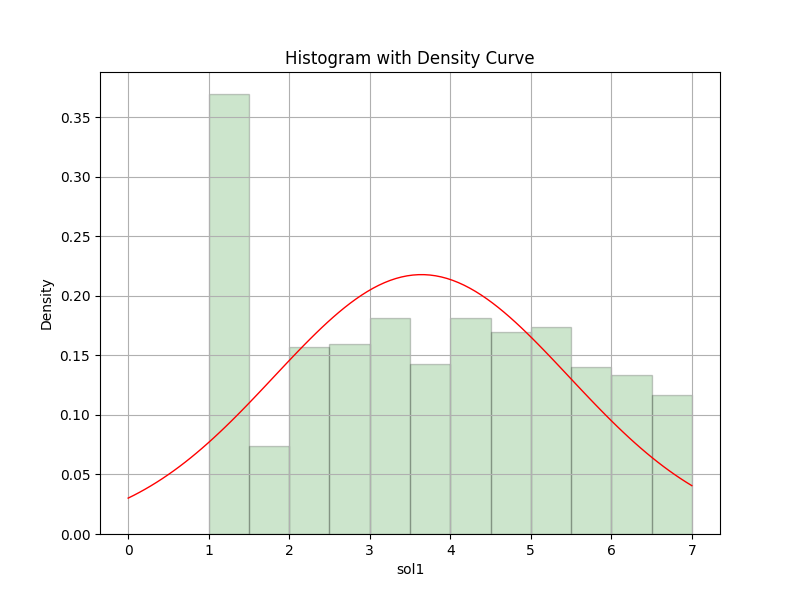
\includegraphics[width=4.06111in,height=2.68611in]{img/histogramaConCurvaDeDensidad.png}
    \caption{Histograma con Curva de Densidad}
    \label{fig:hist_density}%
\end{figure}%


La figura \ref{fig:hist_density} muestra este tipo de gráfico correspondiente a los datos analizados.

En el eje Y se presentan los valores de densidad que van desde 0.00 hasta aproximadamente 0.35, representando la densidad de la variable sol1. Por otro lado, en el eje X se muestran los valores del 0 al 7, que representan las diferentes notas obtenidas en la columna sol1 (solemne 1).

La mayor concentración de datos se encuentra alrededor del valor 0.35 en el eje Y, lo cual indica que la mayoría de las observaciones tienen una nota baja en sol1.

La curva de densidad, representada en color rojo, alcanza su punto más alto entre las notas 3 y 4 en el eje X. Esta curva suavizada muestra la forma general de la distribución de los valores de sol1. A medida que las notas aumentan, la densidad disminuye gradualmente.

En resumen, el análisis del histograma con curva de densidad revela que la mayoría de las observaciones tienen una nota baja en sol1, concentrándose principalmente alrededor del valor 0.35 en el eje Y. Además, la curva de densidad muestra un pico más alto entre las notas 3 y 4 en el eje X.

\subsection{Identificar valores atípicos}

En el análisis de datos, la detección de valores atípicos es crucial para identificar observaciones que difieren significativamente de la tendencia general. Estos valores pueden tener un impacto significativo y requerir atención especial.

A continuación se muestra una tabla con los valores atípicos identificados mediante el método del Z-score. Se calculó el Z-score para cada observación utilizando un umbral de 3 desviaciones estándar. Los valores que superan este umbral se consideran atípicos y se presentan en la tabla:

\begin{table}[htbp]
    \centering
    \caption{Valores Atípicos}
    \begin{tabular}{ccccccc}
        \hline
        \textbf{hito1} & \textbf{hito2} & \textbf{exitosos} & \textbf{fallidos} \textbf{programa} & \textbf{sol1} & \textbf{aprobado}     \\
        21.0           & 6.0            & 17                & 14                                  & UNAB11500     & 1.0               & 0 \\
        2.0            & 2.0            & 4                 & 27                                  & UNAB12210     & 1.0               & 0 \\
        4.0            & 4.0            & 6                 & 41                                  & UNAB12510     & 1.5               & 0 \\
        0.0            & 0.0            & 0                 & 47                                  & UNAB12100     & 1.6               & 0 \\
        10.0           & 6.0            & 9                 & 38                                  & UNAB11500     & 1.6               & 0 \\
        12.0           & 0.0            & 9                 & 38                                  & UNAB12210     & 2.4               & 0 \\
        42.0           & 12.0           & 26                & 37                                  & UNAB21500     & 2.5               & 0 \\
        32.0           & 32.0           & 26                & 5                                   & UNAB11500     & 3.4               & 0 \\
        9.0            & 0.0            & 7                 & 40                                  & UNAB11500     & 4.3               & 1 \\
        38.0           & 6.0            & 28                & 35                                  & UNAB12210     & 4.4               & 1 \\
        32.0           & 32.0           & 26                & 5                                   & UNAB12210     & 4.6               & 1 \\
        18.0           & 2.0            & 11                & 20                                  & UNAB12210     & 4.6               & 1 \\
        32.0           & 14.0           & 21                & 10                                  & UNAB12210     & 5.9               & 1 \\
        13.0           & 25.0           & 16                & 15                                  & UNAB22115     & 7.0               & 1 \\
        7.0            & 0.0            & 5                 & 42                                  & UNAB12100     & 7.0               & 1 \\
        \hline
    \end{tabular}%
    \label{tab:valores_atipicos}%
\end{table}%

Observando los valores atípicos en la tabla \ref{tab:valores_atipicos}, podemos notar que algunas observaciones difieren significativamente en al menos una de las variables. "Exitosos" representa las respuestas correctas de la guía, "Fallidos" indica la cantidad de errores para lograr los "Exitosos", y "Envíos" es la suma de "Exitosos" y "Fallidos". "Sol1" se refiere a la nota obtenida en la solemne 1. Estos valores atípicos pueden ser de interés para un análisis más detallado, ya que podrían indicar situaciones excepcionales o errores en la recolección de datos.